%1/2in left/right margins, 1in top, 1/2 bottom
\documentclass[12pt]{article}
\hbadness=10000
\tolerance=10000
\textheight 9.7in
\textwidth 7.0in
\oddsidemargin -.5in
\topmargin -.5in
\headsep 0in
\headheight 0in
%\pagestyle{empty}
\usepackage{graphicx}
\newcommand{\by}{\mbox{\boldmath$y$}}
\newcommand{\bX}{\mbox{\boldmath$X$}}
\newcommand{\bbeta}{\mbox{\boldmath$\beta$}}

\begin{document}
\hrule
\medskip
\centerline{\textbf{STATISTICS 801 - Section 250}}\hfill \textbf{Fall 2016}
\centerline{\textbf{Homework Assignment 1 - SOLUTION}}
\smallskip
\hrule
\begin{enumerate}
\item 
\begin{itemize}
\item I do not think that a single sample of blood drawn from a calf is representative because there is too much variation in blood depending on where the blood is located in the calf’s body. Some parts of the the body contain blood with more oxygen than others, more red/white cells and platelets, etc. Perhaps several samples from various parts of the body would be more representative - near the skin surface, deep in the stomach, close to an open wound, etc. This sample would represent the blood of the chosen calf within the area of the puncture.
\item The needles could potentially be a representative sample, depending on how many needles are selected, how they are selected, and the natural variation in these needles.
\item The denim is certainly not representative because a bolt of denim fabric can only come from one factory at one time and only be one color while denim can be any color and come from factories all around the world. A more representative sample would be pieces of randomly selected bolts from randomly selected factories and randomly selected batches. This sample is representative of this bolt of denim cloth - and perhaps of other bolts of denim cloth in this same batch, depending on batch production set-up.
\item  The drivers are a terrible sample because the streets of Nebraska are filled with young teenage drivers and out-of-state drivers - neither category fits into the sample. A more representative sample might be 1,000 drivers randomly selected from randomly selected locations throughout the state at randomly selected times of day and week. This sample represents the population of drivers with Nebraska licenses who got their licenses about 10 years before July 1, 2003.
\item The millet plants are not representative of the whole field, necessarily. For example, if this row is flush against a wall, it may get the least amount of sun and the least amount of wind. This sample is representative, however, of that row of millet plants.
\end{itemize}
\item 
\begin{itemize}
\item[a.] The first variable in the data set is HEN. It is qualitative and nominal (might as well have named them Mary, Sarah, and Jane). \\
The second variable in the data set is EGGNO and it is quantitative and discrete. \\
The third variable is EGGWT. It is also quantitative and it is continuous because the average egg weight could potentially take on any real value (within the range of 40-65, apparently).\\
The final variable is FEEDC and it is quantitative and continuous because it could take on any real value.
\item[b.] We know that the population mean egg weight is $\frac{53.4+59.4+53.6+46.3+56.8+51.4+53.9+48.7+55.2+59.5+48.1+61.9}{12}=\frac{648.2}{12}=54.016$. \\
 If a sample of 4 hens were randomly selected from the 12, we would expect the sample mean egg weight to be about the same as the population mean egg weight or the mean egg weight. Since only one hen had a mean egg weight of 61.9 (or, in fact, of above 60 at all), we know that his sample must actually have been that hen four times (perhaps he just caught the slowest hen each time and that was the same creature — a slow runner because of her heavy eggs!). This is highly suspicious since the probability of drawing that same hen four times is $\left(\frac{1}{12}\right)^4=\frac{1}{12^4}=\frac{1}{20736}$.
 \item[c.] Be careful! Your selections are probably different!\\
 I randomly selected hens 31, 38, 33, and 47. Their egg weights are 51.4, 55.2, 53.9, and 61.9, respectively. The sample mean for this sample is $\frac{51.4+55.2+53.9+61.9}{4}=\frac{222.4}{4}=55.6$.\\
 Another sample: hens 47, 38, 25 and 30. Their egg weights are 61.9, 55.2, 53.4, and 56.8, respectively. The sample mean for this sample is $\frac{61.9 + 55.2 + 53.4 + 56.8}{4}=\frac{227.3}{4}=56.825$.\\
 Both of these means are higher than the population mean and different from each other, but they are close (54, 55, and 56). This makes sense because the sample means are just estimates and each estimate will approximate the population mean, but will not give the exact population mean (usually) and will give just one sample mean not every sample's mean.
 \item[d.] We know that $s^2=\frac{\textstyle \sum_{i=1}^n (x_i-\bar{x})^2}{n-1}$, where n=4, and $\bar{x}$ is the sample mean or $\frac{\sum_{i=1}^n x_i}{n}=55.6$ as we calculated in part c. Then\\
 $s^2=\frac{\textstyle \sum_{i=1}^4 (x_i-55.6)^2}{3}$\\
 $=\frac{(51.4-55.6)^2 + (55.2-55.6)^2 + (53.9-55.6)^2 + (61.9-55.6)^2 }{3}$\\
 $=\frac{(-4.2)^2 + (-0.4)^2 + (-1.7)^2 + (6.3)^2}{3}$\\
 $=\frac{17.64 + 0.16 + 2.89 + 39.69}{3}\frac{60.38}{3}=20.126$.\\
 We see that $\hat{\sigma}^2=s^2=20.126$ approximates $\sigma^2=21.714$, as desired.
 \item[e.]
  When we chose the two samples of 4 hens from part (b) we essentially picked a hen, recorded the information, and put the hen back - four times. This means that, with a nonzero probability, we could have picked the same hen each time, like the guy in part (b). To avoid any chance of this happening, we could have picked a hen, recorded the information, and put the hen in a different pen - four times. This means that after we've picked a hen once, that hen can never be picked again in this sample.
\end{itemize}
\item
\begin{itemize}
\item[a.]   First we order the weights from smallest to largest: 889, 893, 895, 902, 909. 
The mean is $\bar{x}=\frac{909+902+893+889+895}{5}=897.6$\\
The median is $895$. i.e., the middle data point (or the average of the middle two if there is an even number of data points).\\
The range is is the largest weight minus the smallest weight; $R=909-889=20$.\\
The population variance is estimated by the sample variance \\
$s^2=\frac{\textstyle \sum_{i=1}^n (x_i-\bar{x})^2}{n-1}$\\
$=\frac{\textstyle \sum (x-897.6)^2}{4}$\\
$=\frac{(909-897.6)^2 + (902-897.6)^2 + (893-897.6)^2 + (889-897.6)^2 + (895-897.6)^2 }{4}$\\
$=\frac{(11.4)^2 + (4.4)^2 + (-4.6)^2 + (-8.6)^2 + (-2.6)^2}{4}$\\
$=\frac{129.96 + 19.36 + 21.16 + 73.96 + 6.76}{4}$\\
$\frac{251.2}{4}=62.8$.\\
The population standard deviation is estimated by the sample standard deviation $s=\sqrt{s^2}=\sqrt{62.8}=7.9246$.\\
The standard deviation of the mean is estimated by the standard error of the mean$SD_{\bar{X}}=\frac{s}{\sqrt{n}}=\frac{\sqrt{62.8}}{\sqrt{5}}=3.5440$.\\
The coefficient of variation of slaughter weight is $cv=\frac{\sigma}{\mu}$, and it is estimated by $\hat{cv}=\frac{s}{\bar{x}}=\frac{\sqrt{62.8}}{897.6}=0.0088$.
\item[b.]  $\sum_{i=1}^5(x_i-\bar{x})=(909-897.6) + (902-897.6) + (893-897.6) +(889-897.6) + (895-897.6) $\\
$=(11.4) + (4.4) + (-4.6) + (-8.6) + (-2.6) = 15.8-15.8 = 0. $\\
 We see here that this holds true for any data set:\\
  $\sum_{i=1}^n(x_i-\bar{x})=(x_1-\bar{x})+(x_2-\bar{x})+...+(x_n-\bar{x})$\\
  $=x_1+x_2+...+x_n-n\bar{x}$\\
  $=x_1+x_2+...+x_n-n\left(\frac{x_1+x_2+...+x_n}{n}\right)$\\
  $=x_1+x_2+...+x_n-(x_1+x_2+...+x_n)$\\
  $=x_1+x_2+...+x_n-x_1-x_2-...x_n=0$\\
  If something is always 0, it does not tell us anything about the dispersion of the data, thus the average deviation about the mean is not a useful measure of dispersion. This makes sense, however, when one thinks about the fact that the mean is the average of all the data points and dispersion is the difference between a data point and the mean. Therefore, the mean dispersion is the average difference between a data point and the average of all data points which should be 0.
\item[c.]  First we subtract 900 from each of the weights from smallest to largest: 889-900=-11, 893-900=-7, 895-900=-5, 902-900=2, 909-900=9. \\
The mean is $\mu\approx\bar{y}=\frac{-11 +(-7) +(-5) + 2 + 9 }{5}=\frac{-12}{5}=-2.4=897.6-9000=\bar{x}-900$,  i.e., the population mean is $\mu$ and it is estimated by the sample mean $\bar{y}=\bar{x}-900$.\\
The population variance is $\sigma^2=\frac{\sum(y-\mu)^2}{N}$, and it is estimated by the sample variance\\
$s^2=\frac{\sum(y-\hat{y})^2}{n-1}$\\
$=\frac{\sum(y+2.4)^2}{4}$\\
$=\frac{(-11 + 2.4)^2 + (-7 + 2.4)^2 + (-5 + 2.4)^2 + (2 + 2.4)^2 + (9 + 2.5)^2 }{4}$\\
$=\frac{(-8.6)^2 + (-4.6)^2 + (-2.6)^2 + (4.4)^2 + (11.4)^2}{4}$\\
$=\frac{73.96 + 21.16 + 6.76 + 19.36 + 129.96}{4}=\frac{251.2}{4}=62.8$.\\
We see that subtracting 900 from each of the weights is equivalent to subtracting 900 from the mean calculated in part (a). We also see that subtracting 900 from each of the weights did not change the variance from what we calculated in part (a). This leads us to believe that a shift in the data points (one that is consistent for each data point, i.e., adding or subtracting a constant to/from each value) will produce an equivalent shift in the mean, but not have any effect on the variance. These results could be used to make our computations easier by working with smaller numbers to compute the shifted mean and the variance by shifting all data points and then un-shifting or adding the negative of the constant to the new mean to produce the original mean - and using the variance as-is.
\end{itemize}
\item
\begin{itemize}
\item[a.]$Q(0.05)=?$\\
$p=0.05 \;\;\;\; p_i=0.0375 \;\;\;\; n=40 \;\;\;\;  Q(p_i)=9 \;\;\;\; Q(p_{i+1})=9$\\
$f=n(p-p_i)=40(0.05-0.0375)=40(0.0125)=0.5$\\
$Q(p)=(1-f)Q(p_i)+fQ(p_{i+1})$\\
$Q(0.05)=(1-0.5)9+0.5\cdot9=0.5\cdot9+0.5\cdot9=9$\\[0.1in]
$Q(0.333)=?$\\
$p=0.333 \;\;\;\; p_i=0.3125 \;\;\;\; n=40 \;\;\;\; Q(p_i)=14 \;\;\;\; Q(p_{i+1})=16$\\
$f=n(p-p_i)=40(0.333-0.3125)=40(0.0205)=0.82$\\
$Q(p)=(1-f)Q(p_i)+fQ(p_{i+1})$\\
$Q(0.333)=(1-0.82)14+0.82\cdot16=0.18\cdot14+0.82\cdot16=15.64$\\[0.1in]
$Q(0.45)=?$\\
$p=0.45 \;\;\;\; p_i=0.4375 \;\;\;\; n=40 \;\;\;\; Q(p_i)=23 \;\;\;\; Q(p_{i+1})=24$\\
$f=n(p-p_i)=40(0.45-0.4375)=40(0.0125)=0.5$\\
$Q(p)=(1-f)Q(p_i)+fQ(p_{i+1})$\\
$Q(0.45)=(1-0.5)23+0.5\cdot24=0.5\cdot23+0.5\cdot24=23.5$\\[0.1in]
$Q(0.8)=?$\\
$p=0.8 \;\;\;\; p_i=0.7875 \;\;\;\; n=40 \;\;\;\; Q(p_i)=46 \;\;\;\; Q(p_{i+1})=47$\\
$f=n(p-p_i)=40(0.8-0.7875)=40(0.0125)=0.5$\\
$Q(p)=(1-f)Q(p_i)+fQ(p_{i+1})$\\
$Q(0.8)=(1-0.5)46+0.5\cdot47=0.5\cdot46+0.5\cdot47=46.5$\\[0.1in]
$Q(0.8925)=?$\\
$p=0.8925 \;\;\;\; p_i=0.8875 \;\;\;\; n=40 \;\;\;\;  Q(p_i)=61 \;\;\;\; Q(p_{i+1})=65$\\
$f=n(p-p_i)=40(0.8925-0.8875)=40(0.005)=0.2$\\
$Q(p)=(1-f)Q(p_i)+fQ(p_{i+1})$\\
$Q(0.8925)=(1-0.2)61+0.2\cdot65=0.8\cdot61+0.2\cdot65=61.8$
\item[b.] In the boxplot the 5 horizontal lines (left to right) represent:
\begin{enumerate}
\item[1.] Lower fence = $Q_1-1.5IQR$=12.5-34.5=-22
\item[2.] Q1=12.5
\item[3.] Q2=median=26
\item[4.] Q3=35.5
\item[5.] Upper fence = $Q_3+1.5IQR$=35.5+34.5=70
\end{enumerate}
The 2 dots (on the right - outside of the upper fence) represent the outliers (outside values); namely 94 and 110.
%\begin{center}
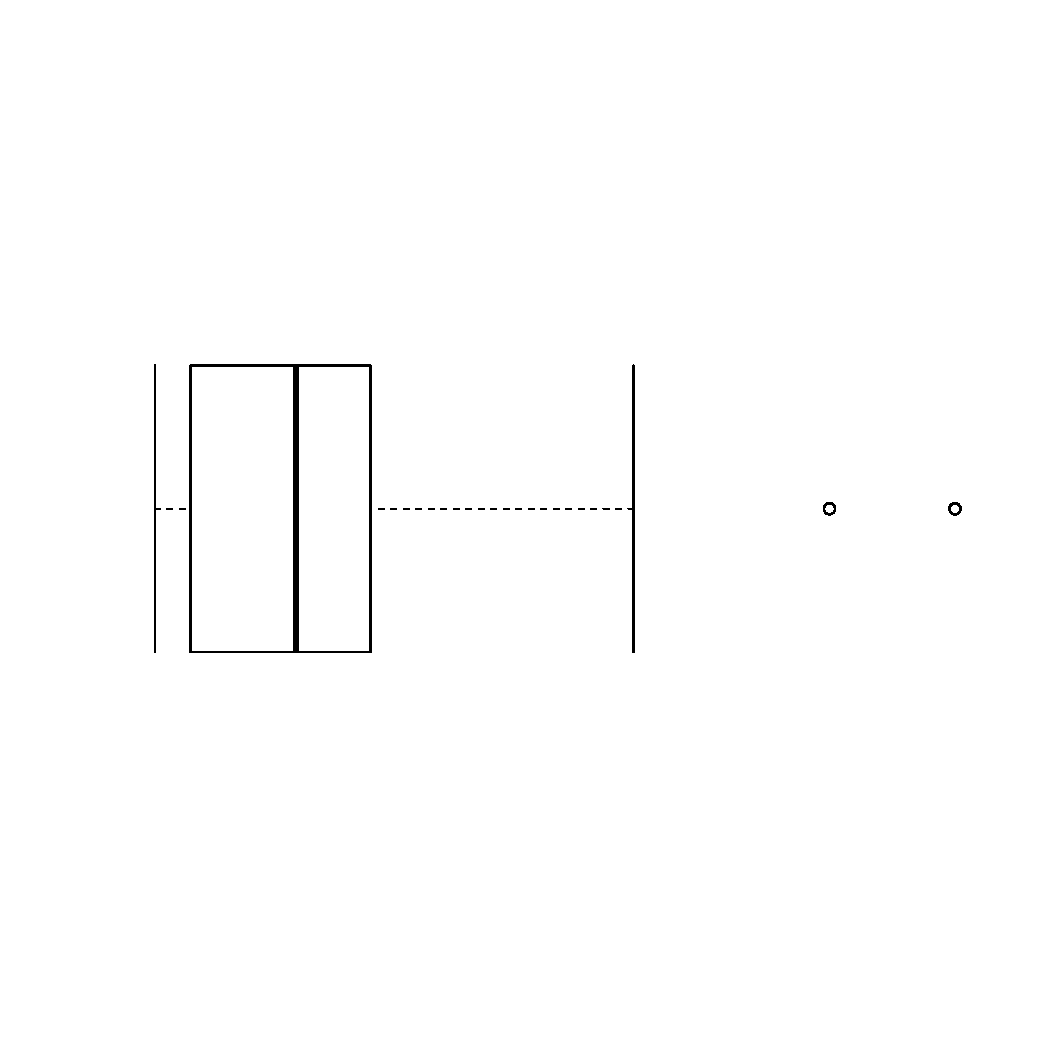
\includegraphics[scale=0.2]{boxplot.pdf}
%\end{center}
\end{itemize}
\item 
\begin{itemize}
\item[a.] The population consists of the responses of all adults in the United States, and the sample consists of the responses of the 1708 adults in the United States in the survey.
\item[b.] The population consists of the prices per gallon of regular gasoline at all gasoline stations in the United States, and the sample consists of the prices per gallon of regular gasoline at the 800 surveyed stations.
\end{itemize}

\item 
\begin{itemize}
\item[a.] Because the average of $\$122,000$ is based on a subset of the population, it is a sample statistic.
\item[b.] Because the percent increase of $8.5\%$ is based on all 667 graduates' starting salaries, it is a population parameter.
\end{itemize}
\end{enumerate}
\newpage
EXTRA CREDIT:\\
$\sum_{i=1}^n(x_i-\bar{x})^2=\sum_{i=1}^n(x^2_i-2\bar{x}x_i+\bar{x}^2)=\sum_{i=1}^nx^2_i-2\bar{x}\sum_{i=1}^nx_i+\sum_{i=1}^n\bar{x}^2$\\
$\sum_{i=1}^nx^2_i-2\bar{x}n\frac{\sum_{i=1}^nx_i}{n}+\bar{x}^2\left(\sum_{i=1}^n1\right)$\\
$=\sum_{i=1}^nx^2_i-2\bar{x}n\bar{x}+\bar{x}^2(n)$\\
$=\sum_{i=1}^nx^2_i-2n\bar{x}^2+n\bar{x}^2=\sum_{i=1}^nx^2_i-n\bar{x}^2$\\
$=\sum_{i=1}^nx^2_i-n\left(\frac{\sum_{i=1}^nx_i}{n}\right)^2$\\
$=\sum_{i=1}^nx^2_i-n\frac{\left(\sum_{i=1}^nx_i\right)^2}{n^2}$\\
$=\sum_{i=1}^nx^2_i-\frac{\left(\sum_{i=1}^nx_i\right)^2}{n}$.


\end{document}

